%update: Dec 20 wrote more
%update: Nov 09 Prof checked some of the texts

\begin{savequote}[75mm] 
There's plenty of room at the bottom.
\qauthor{Richard Feynman} 
\end{savequote}

\chapter{Introduction}
\newthought{The} advancement of material science and technology has led to the discovery and utilization of nanoscale materials. Many of these new materials possess extraordinary chemical, electrical, optical or mechanical properties. However, as human beings, who are millions or billions times larger than nanomaterials, we are not eligible to reach them directly. As Feynman said, there is plenty of possibility at the bottom, but it also means that plenty of efforts are expected for researching. 

\begin{figure}  
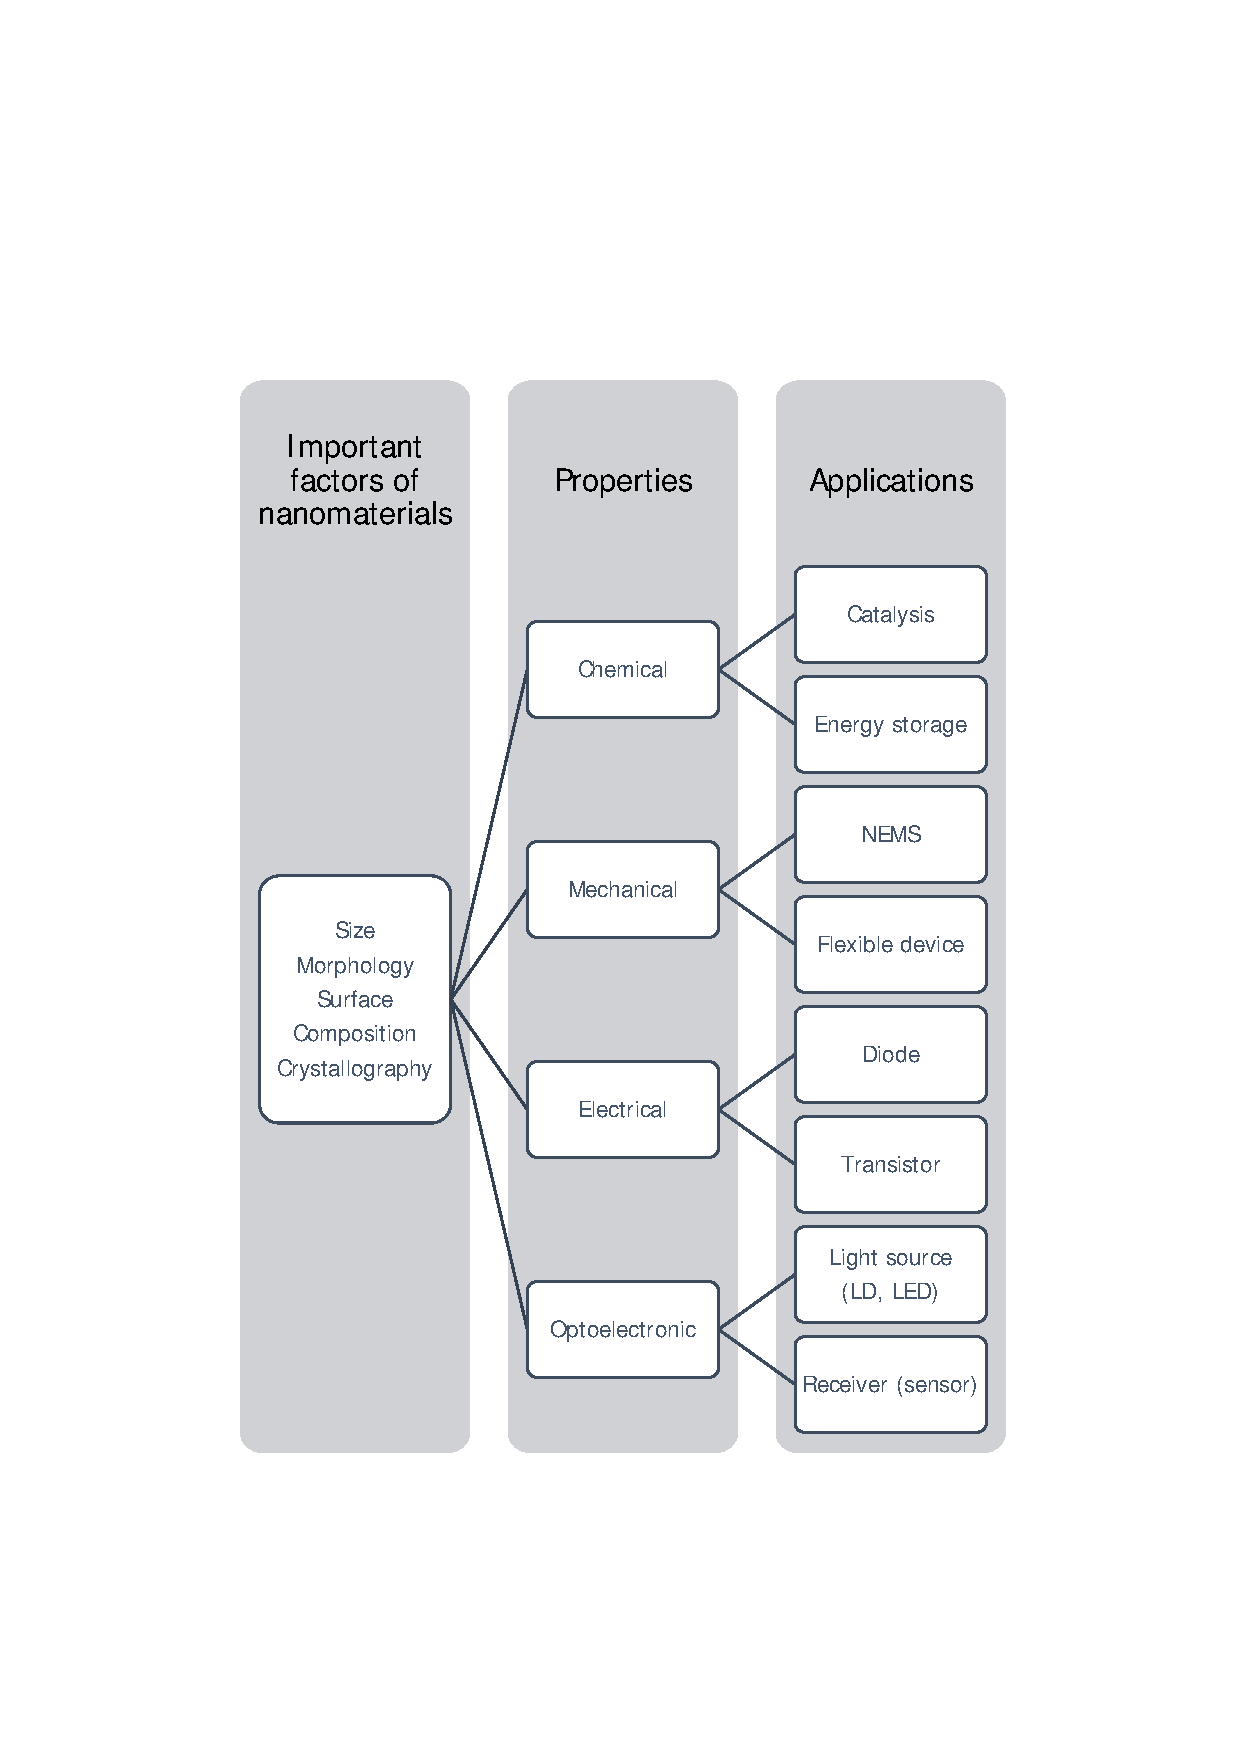
\includegraphics[width=320pt]{figures/figure1_factors}
\caption[Factors and applications]{The special factors of nanomaterials contribute to various applications. 
\label{fig:1_factor}}
\end{figure}

%nanoscale--nanomaterials--to see--to manipulate
\section{Probing on nanomaterials}
%what is nanomater...why nanomater...
Generally, nanomaterials are materials in which a single unit is sized from one nanometer to a few hundreds of nanometers. The scale difference between these materials and human body is more than a million. Besides scale difference, nanostructures usually process special properties as compared with bulk materials due to chemical composition difference, surface to volume ratio and quantum confinements. The confined structures of the same chemical type and composition might present very different properties. An easy way to understand a value of the nanomaterial is to consider carbon materials. We know diamond and graphite are allotropes of carbon which possess different bonding and thereby amazingly distinct physical and chemical characteristics. This is also true for fullerene, carbon nanotube and graphene. Even the number of walls in a carbon nanotube would significantly affect its properties. \cite{rodunerwhynano2006} Therefore, what makes nanostuctures distinctive is not only the size, but also their unique compositions, surface effects and quantum confinement effects. 

\renewcommand{\thefootnote}{\fnsymbol{footnote}}

As shown in Figure \ref{fig:1_factor}, all effects contribute to the particular functionality of a nanomaterial. Such as superior mechanical strength and rigidity, ultrahigh electrical mobility, abundant chemical active sites, ect. Mechanical superiority is important for mechanical applications such as flexible electronics and devices in Nano Electro Mechanical Systems (NEMS). Electrical superiority of nanomaterials with various electrical band structures could be applied to diodes, transistors, laser diodes (LDs), light-emitting diode (LEDs) in transparent or flexible electronics and optoelectronics. Chemical superiority of nanomaterials made them desired for high efficiency catalysis and portable energy storage devices with high energy density. 

%limitations to study nanomater...

\begin{figure} 
\centering
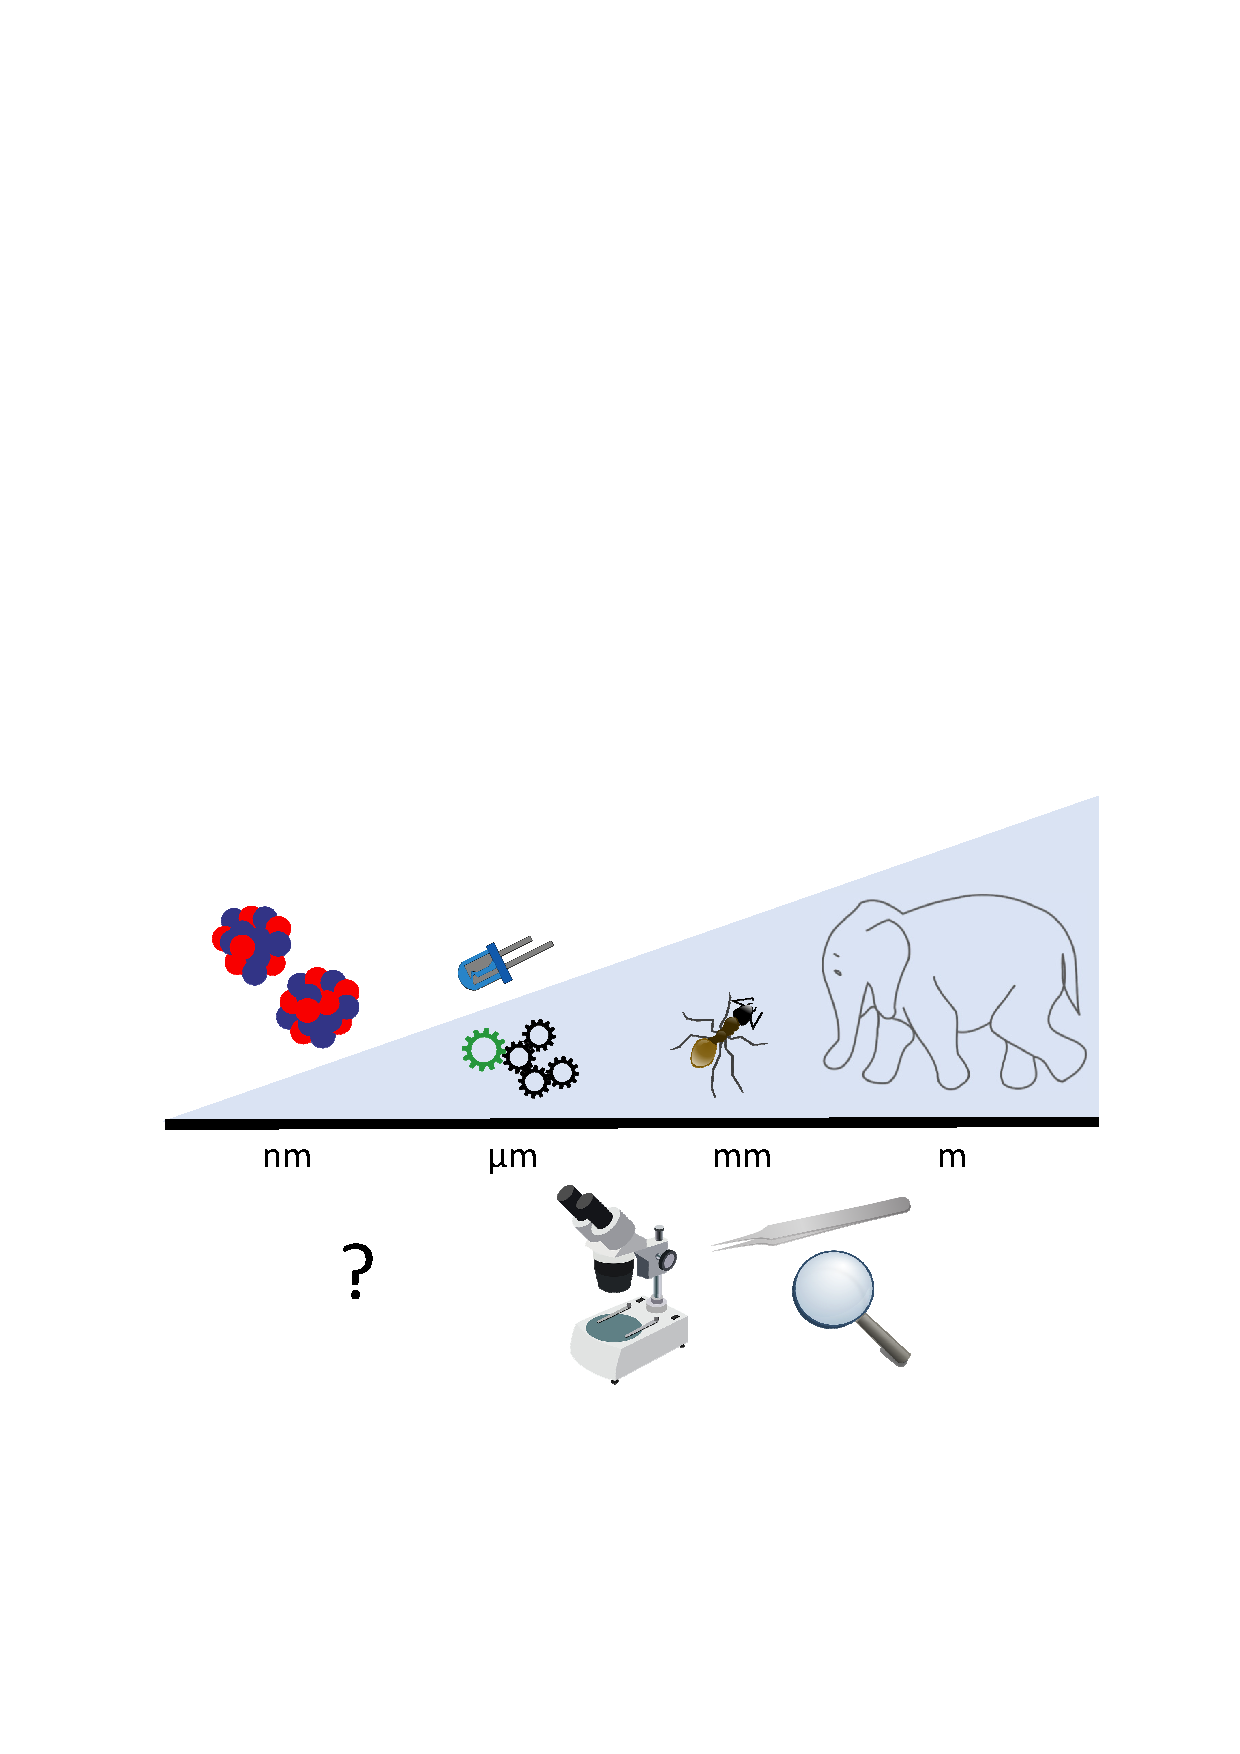
\includegraphics[width=350pt]{figures/figure1_scale_problem.pdf}
\caption[Scale problem]{How human beings gain access to lower scales, to see and to manipulate.\footnotemark[1]
\label{fig:1_scale}}
\end{figure}

However, it is not straightforward to access the properties of these nanomaterials and prepare them for real applications, unfortunately, also due to the same reason - small scale. We understand that the observation, reach and built of an object which is $10^6$ to $10^9$ (in one dimension) smaller then real world macro-objects, for example the {\em Great Wall of China} ($21,196 km$), is challenging. Similarly, as compared with human beings' hands of whose size is about $20 cm$, nanoscaled objects are usually million times smaller. Hence, even the nanoscale building blocks are superior, we are not able to utilize them easily. As shown in Figure \ref{fig:1_scale} \footnote{Without specification, all clip art materials (elephant, ant, microscope, tweezers, etc.) in figures of the dissertation are adapted from Internet which are {\em free to use without attribution}.}, we are able to reach smaller scales by tweezers and optical microscopes, but it is challenging to reach nanoscale objects. 

%introduce to microscopy and probing tech. 
The way human beings make use of fire, tools and even light and electrons is perhaps what sets our modern lives above of other species. By understanding and utilizing photons, electrons and atomic forces, microscopy allows us to view sub-millimeter objects that cannot be observed with a naked eye. Thanks to the advancement of tools - microscopy and piezoelectric material - we can now access to nanomaterials by high precision probing technique with direct high-resolution observation. By applying electric field on a piece of piezoelectric material, the material change shape in function of the electric field precisely. Therefore we might control the movement by electrical biases and confirm location of object and probe by microscopy. 

%what is in situ TEM
\section{Seeing is believing: Transmission Electron Microscopy}
In the past centry, development of particle physics make way for new microscopies such as Scanning Probe Microscopy (SPM, including Atomic Force Microscopy and Scanning Tunneling Microscopy), Scanning Electron Microscope (SEM), and Transmission Electron Microscopy (TEM). Among all microscopies, transmission electron microscopy (TEM), is the ultimate resolution tool that allows one to reach atomic resolution with full crystallography information. TEM provides deep and direct information from a thin sample by the transmission and diffraction of electrons. 

\begin{figure}  
\centering
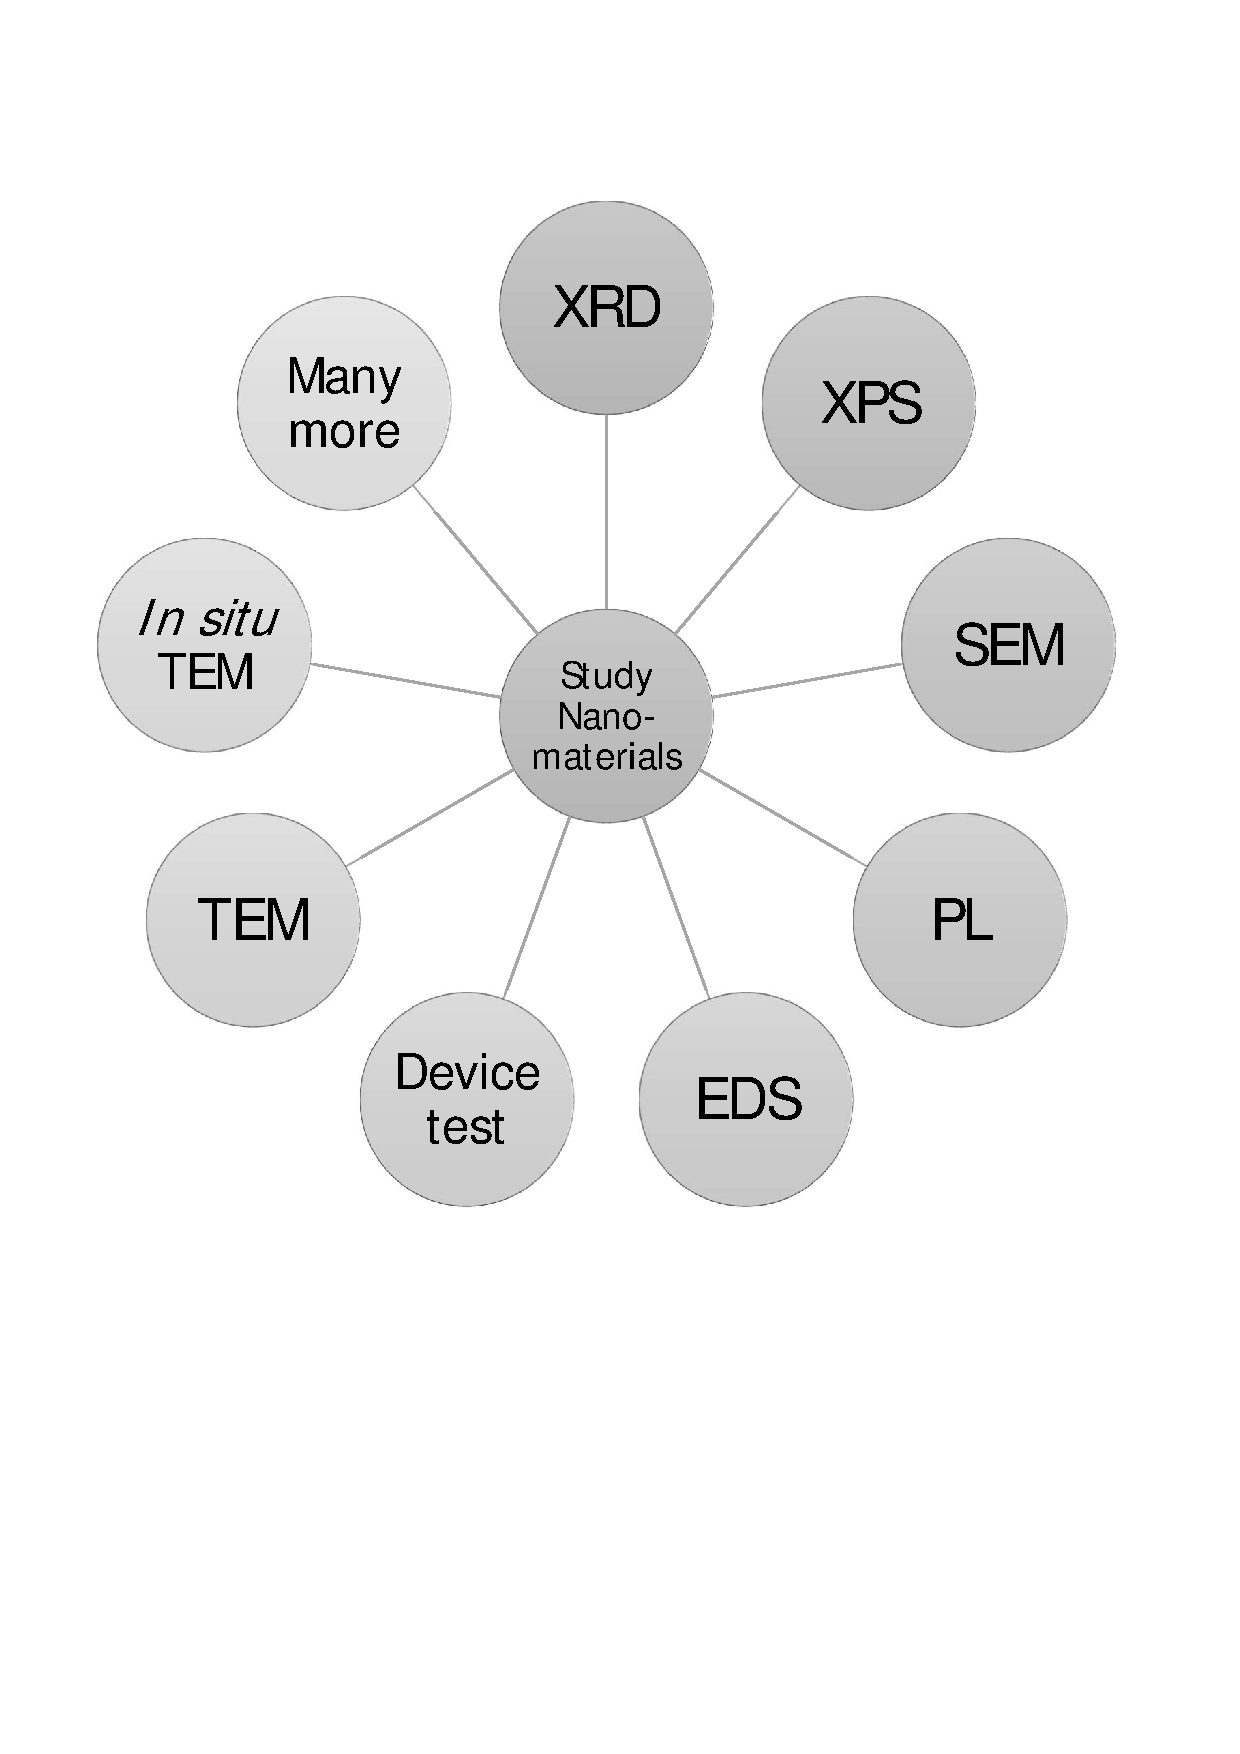
\includegraphics[width=300pt]{figures/figure1_to_study_nanomater.pdf}
\caption[To study nanomaterials]{{\em In situ} TEM serves as a way to study nanomaterials.
\label{fig:1tsn}}
\end{figure}

When researchers are not satisfied with only seeing of static material, dynamics was introduced to the sample. \emph{In situ} transmission electron microscopy(TEM) is the newest advanced technology which gives access to the sample dynamics via observation, manipulation and various tests. Particularly, by adapting the microscope or using a special specimen holder, it is possible to make deliberate attempts to modify materials during high-resolution characterizations. It allows for the observation of dynamic properties of a material under special circumstances. \cite{banhart2008situ}For instance, a heating holder would provide the desired high temperature to trace (by a fast CCD video camera) and thereby reveal chemical transformations within a sample. By contrast, without \emph{in situ} heating, we are only able to see the initial and final states of the reaction; in this way the regarded mechanism is usually inferred based on a few indirect clues, such as X-ray Diffraction (XRD), X-ray photoelectron spectroscopy (XPS), Energy Dispersive X-ray Spectrometry (EDS), Photoluminescence (PL) and indirect TEM characterizations before and after the dynamics. As illustrated in Figure \ref{fig:1tsn}, \emph{in situ} TEM is very important and irreplaceable approach to study nanomaterials. 

\begin{figure}  
\centering
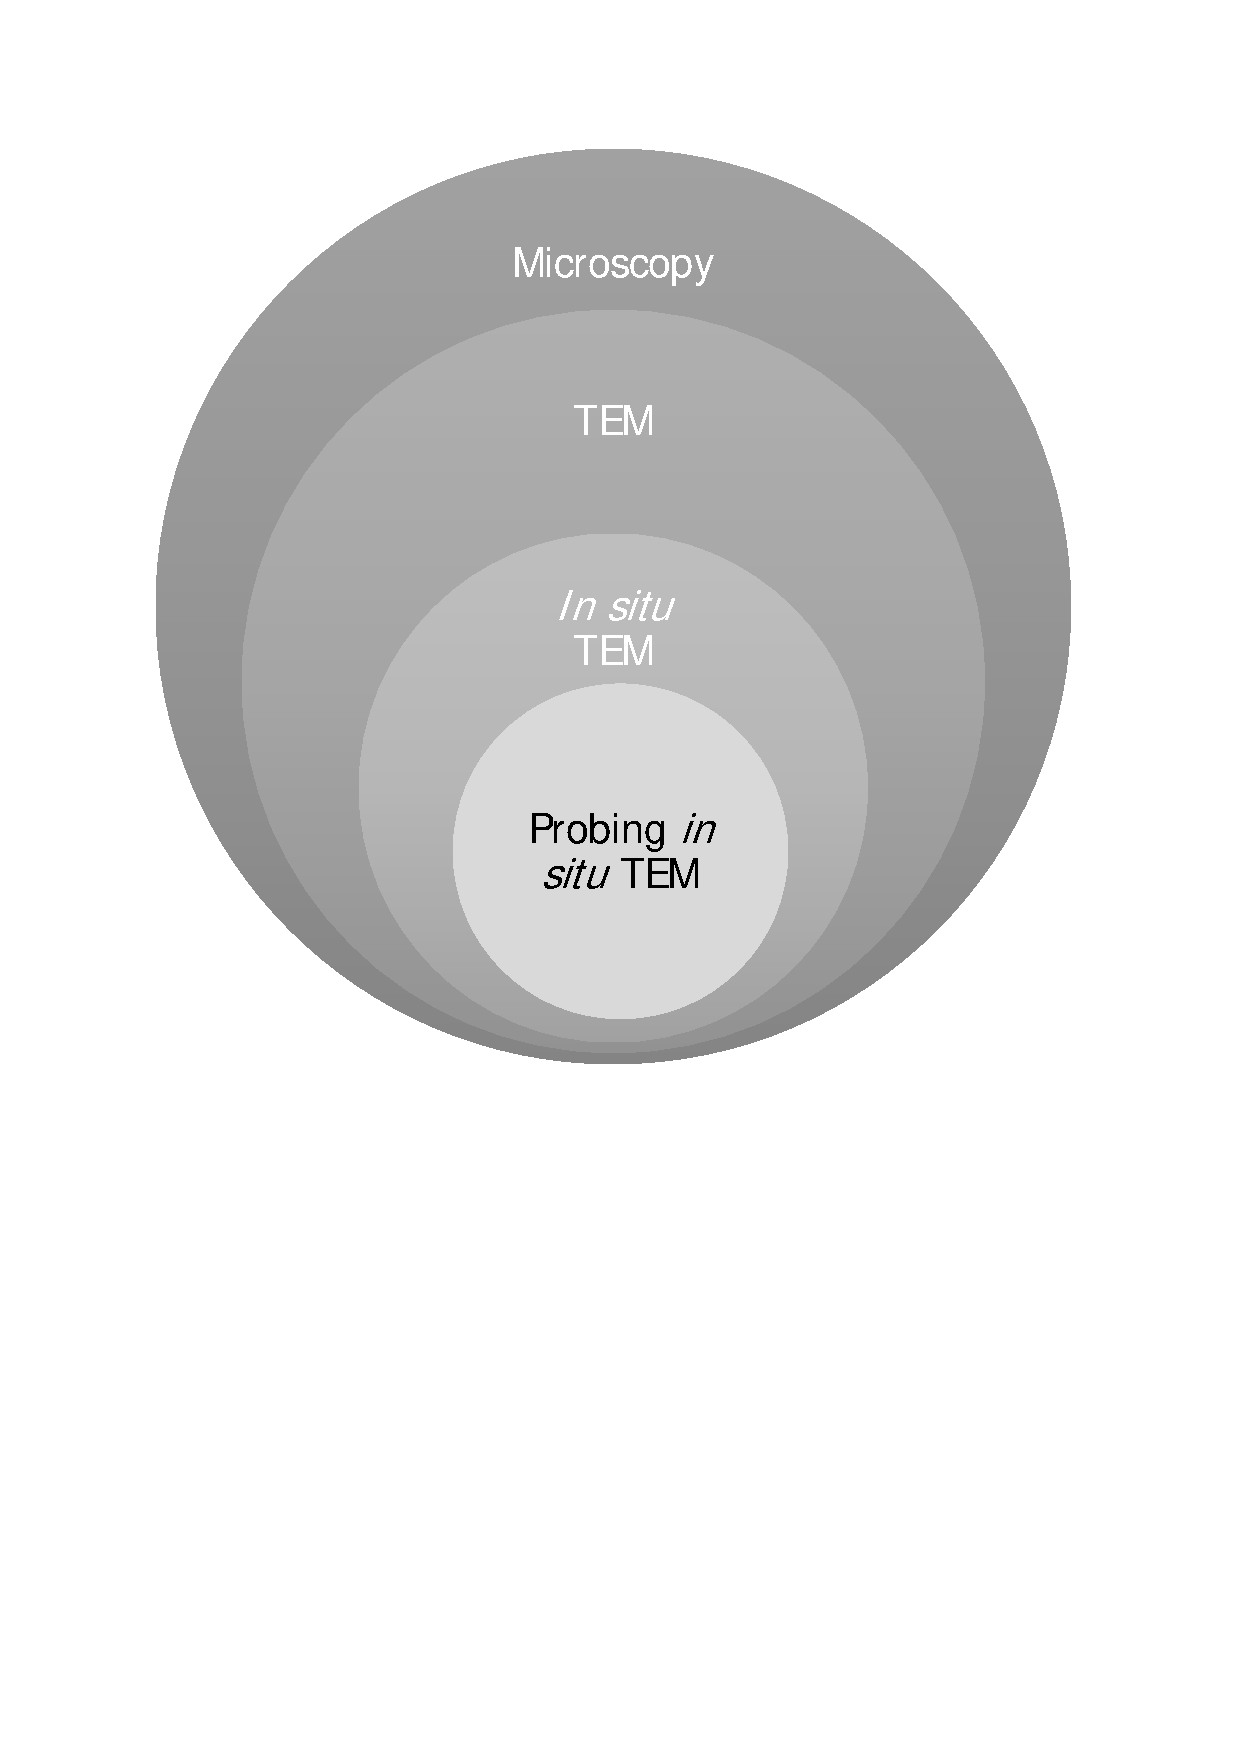
\includegraphics[width=240pt]{figures/figure1_TEM_As_Microscopy.pdf}
\caption[\emph{In situ} TEM as a microscopy]{Relationships between probing \emph{in situ} TEM and other microscopies.
\label{fig:1tam}}
\end{figure}

Various specimen holders make it possible to introduce heating, cooling, electrical bias, mechanical force, gas, liquid, magnetic field, light etc. to the sample under various circumstances. As illustrated in Figure \ref{fig:1tam}, probing \emph{in situ} TEM is one small part of microscopy. This Dissertation is mainly focused on probing of nanomaterials via \emph{in situ} TEM. 

%probing in situ TEM
\section{Untouchable scale: Probing techniques on nanomaterial}

Experiments performed by \emph{in situ} probing microscopy, is performed based on piezoelectric probing technique and microscopy. \\
Piezoelectricity is a phenomenon where electricity is directly related to the pressure on the material. In a piezoelectric actuator, special driving signals are applied to a piezoelectric tube in certain directions, and thereby the piezoelectric tube would respond to change shape accordingly.\cite{okada2004piezoelectric,vishnevsky1977piezoelectric} As shown in Figure \ref{fig:1piezo}, when base of the tube is fixed, transverse and axial movements of tube tip would be expressed approximately by
$$\begin{bmatrix}\Delta x\\ \Delta y\end{bmatrix}= \frac{2\sqrt{2}d_{31}}{\pi Dh}L^2\begin{bmatrix}U_{+x}-U_{-x}\\U_{+y}-U_{-y} \end{bmatrix},$$
$$\Delta L= \frac{d_{31}L}{h}V$$
, where $\Delta x$, $\Delta y$ and $\Delta L$ are deflection in $x$, $y$ and axial direction. $U_{+x}-U_{-x}$, $U_{+y}-U_{-y}$ are driving voltages applied to opposite sides of tube (therefore in total four electrodes except base ground electrode).$V$ is voltage applied to all four quadrants. $L$, $D$ and $h$ is lenth, diameter and thickness of the tube. The transverse piezoelectric coefficient $d_{31}$ applies to voltage is very small (about $-10^{-10} \mathrm{m/V}$), and hence the movement can be controlled precisely by biasing. 

\begin{figure}  
\centering
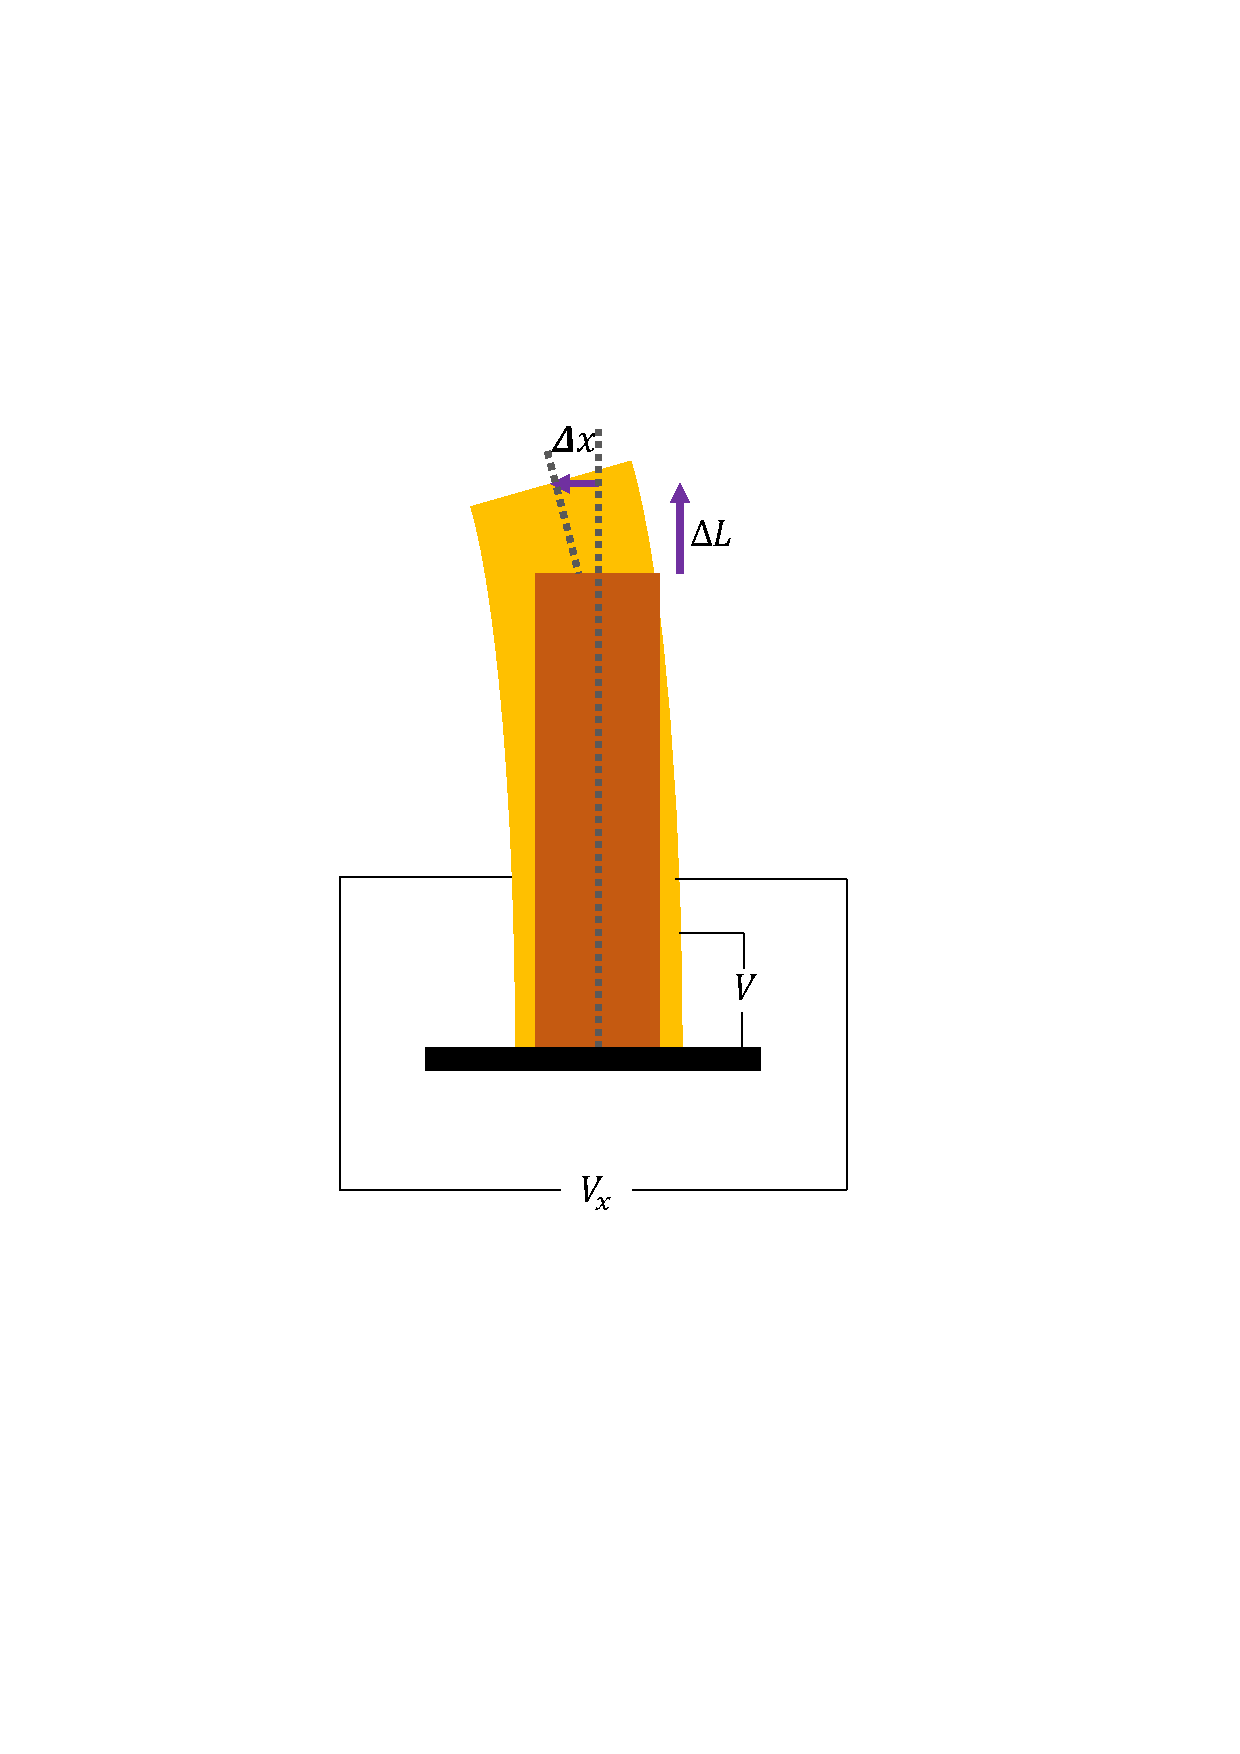
\includegraphics[width=160pt]{figures/figure1_piezo.pdf}
\caption[Probing by piezoelectronics]{Schematic illustration of how piezoelectric works for precised nanomanipulations.
\label{fig:1piezo}}
\end{figure}

With help of a piezoelectric actuator, we can handle a ultrasharp probe to touch the nanoscale sample with nanometer precision. 
\\
Now we have two effective ways to see and touch nanostructures -- {\em in situ} TEM and piezo-motro probing. 


\section{Optoelectronic and flexible electronic applications of nanomaterials}
%light to replace electrons
We are currently fully enjoying the benefits of well developed microelectronics and nanoelectronics. However, people are trying to improve speed of information by means of light. As compared with electrons in metal(copper or even gold) conductors, photons in optical system process much higher capacity of information. The society benefit a lot from optical fiber information technology. For instance, it was quite difficult and expansive to perform high-definition video streaming via Internet 20 years ago when we were using copper wires to transmit electrical information. 
%silicon is not best for optoelectronics
The silicon-based electronics is efficient mainly based on the two materials: silicon and copper(or other conductors such as gold). The manufacturers are sophisticated with etching silicon chips and applying mask for electrode coating. Silicon is absolutely a decent semiconducting material. By doping techniques and smart designs, billions of transistors could work at high speed in a nail-sized chip. The problem is, for optoelectronic applications, band-gap diversity is required. Therefore silicon, as a perfect semiconductor for electronics, could not realize full functioning optoelectronics. \\ 
%silicon is not best for flexible electronics
Besides, flexible electronics attract great attention. In the last few years, we experienced an explosion of flexible optoelectronic applications in flat-panel displays, lighting, sensing, and energy cells. For instance, organic light-emitting diode (OLED) and flexible lithium-ion batteries are developed as a next-generation technology for wearable electronics, bendable smartphones, foldable displays, etc. However, to make silicon wafers flexible is never easy. Therefore, people believe bottom-up technology would arichitect nanoscale building blocks on flexible substrate as future flexible electronics and optoelectroncs. \\

\begin{figure}  
\centering
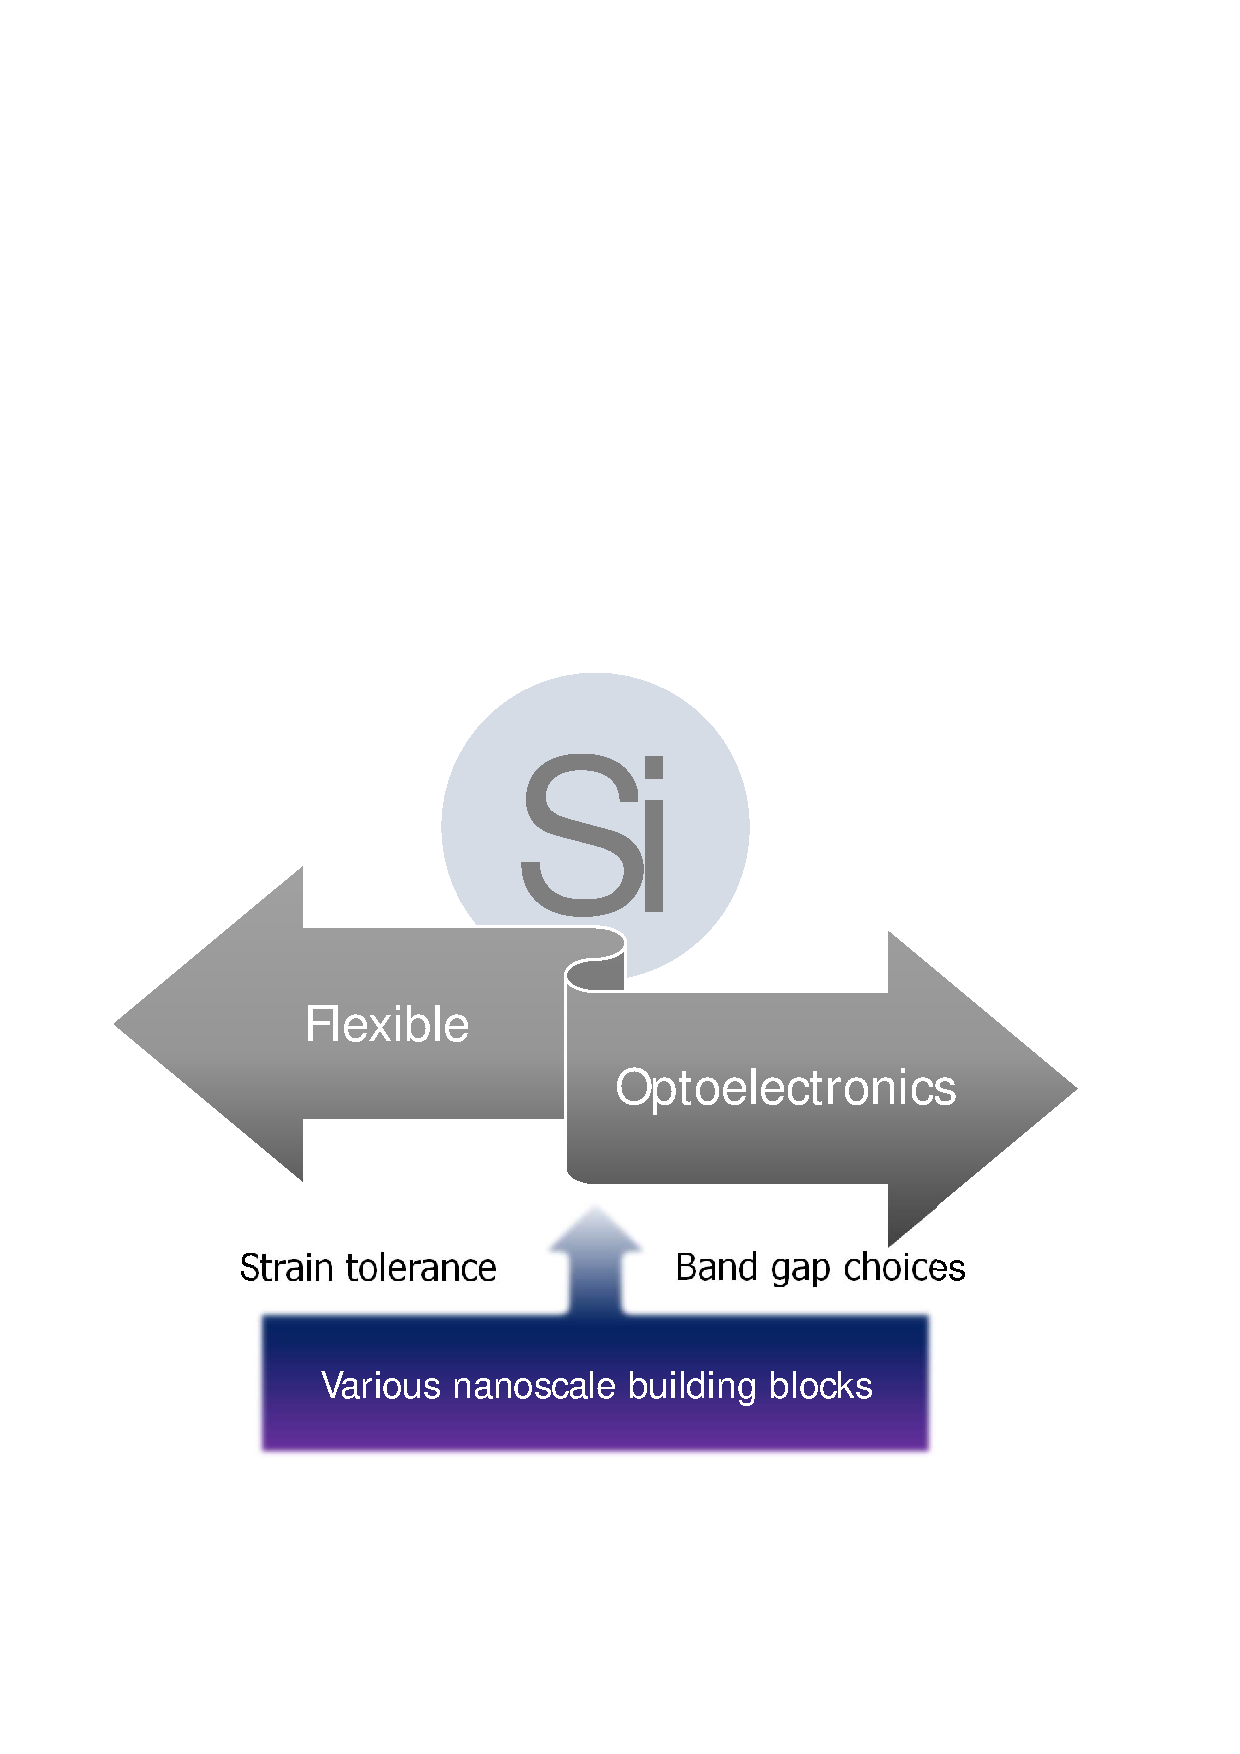
\includegraphics[width=280pt]{figures/figure1_silicon.pdf}
\caption[Future of optoelectronics and flexible electroncis]{Silicon's two short-backs for flexible devices and optoelectronics could be backed-up by bottom-up approach using nanomaterials in future integrations.
\label{fig:1si}}
\end{figure}

%So nanomater is good for optoelectronics and flexible applications
Therefore, for optoelectronic and flexible electronic applications, conventional silicon industries are challenged, as shown in Figure \ref{fig:1si}. Silicon material is an ideal material to meet all requirements by field effect transistors. The silicon based devices are based on controlling carriers realized by structural design and doping. Recent years, silicon-based optoelectronics is growing steadily but not exponentially as expected by Moore's Law. \cite{Waldrop2016} 
The semiconductor industries produce devices mainly by the top-down strategy. A top-down approach is a smart way to apply desired patterns to the device engineering, which came in effect since 1970s, when human beings were not so experienced to manipulate nanostructures. However, these days a bottom-up approach is emerging and shows a high promise to construct systems by piecing building blocks together. It is true that some nanomaterials show superior properties for electronics, but it appears that during the last decade, many effort from various researchers cannot send bottom-up technology to the market. It is expected that in future high quality nanomaterial building blocks could be well handled for device integrating by automated mass production. The integrated LDs, LEDs and photodetectors could be manufactored by nanowires, nanosheets and even quantum dots to realize full functioning optoelectronic chips. The current obstacle is to get more knowledge of the building block materials. How does the electrical signal of nanowires or nanosheets behave under strain and light illumination, what is the photocurrent spectroscopy of the material, such questions are not well studied. Consequently, it is strongly required that we find answers to these questions, in order to provide clues for future flexible electronics and optoelectronics. 

\section{Energy storage applications of nanomaterials}
%energy is important
Electrical energy storage will be far more important nowadays than it was when we have abundant petroleum resources, and when we don't have smart (smart also means energy consuming) electronics. From powering portable electrical devices (cell phones, tablets, laptops), implantable medical applications (pacemaker), to machines (hybrid electric vehicles), the human desire for clean, safe, fast and efficient energy storage is becoming more and more  significant. \\
%ion-batter is important
Among all energy storage applications, lithium ion-batteries (LIBs) are the most required devices due to its high energy density, which is the key factor for portable electronics and automobiles. In LIBs, lithium ions move from the anode to cathode during discharge, and from cathode to anode when charging. The materials for the anode and cathode can dramatically affect a few aspects of the battery’s performance, including stability and capacity. High capacity materials are urgently demanded in order to address the need for greater energy density, cycle life and charge lifespan, among other issues faced by Li-ion batteries. 
%Nanomater for ion-battery
However, conventional materials are well developed but still cannot catch up with the growing demand of battery capacity. Li-ion batteries have struggled with issues such as poor cycle life, rising internal resistance with cycling and age, safety concerns when overheated or overcharged, and growing applications demanding more from capacity. A lot of researches have confirmed that nanomaterials are particularly promising to achieve this target. The advantages are mainly\cite{Bruce2008,qifengzhang2013csr}: \\
\begin{itemize}
	\item[a] Many nanomaterials enable electrode reactions to become reversible while they are not reversible for bulk materials; 
	\item[b] The reduced size significantly increases the rate of energy transformation between electricity to chemicial energy (such as lithiation and delithiation process) due to the short diffusion lengths; 
	\item[c] Electron conductivity can also be improved in nanomaterials; 
	\item[d] High surface to volume ratio provides high contact area between electrodes and electrolyte; 
	\item[e] Chemical potentials of ions and electrons can be different at the nanometer scale, and therefore electrode potential can be modified. 
\end{itemize}

\begin{figure}  
\centering
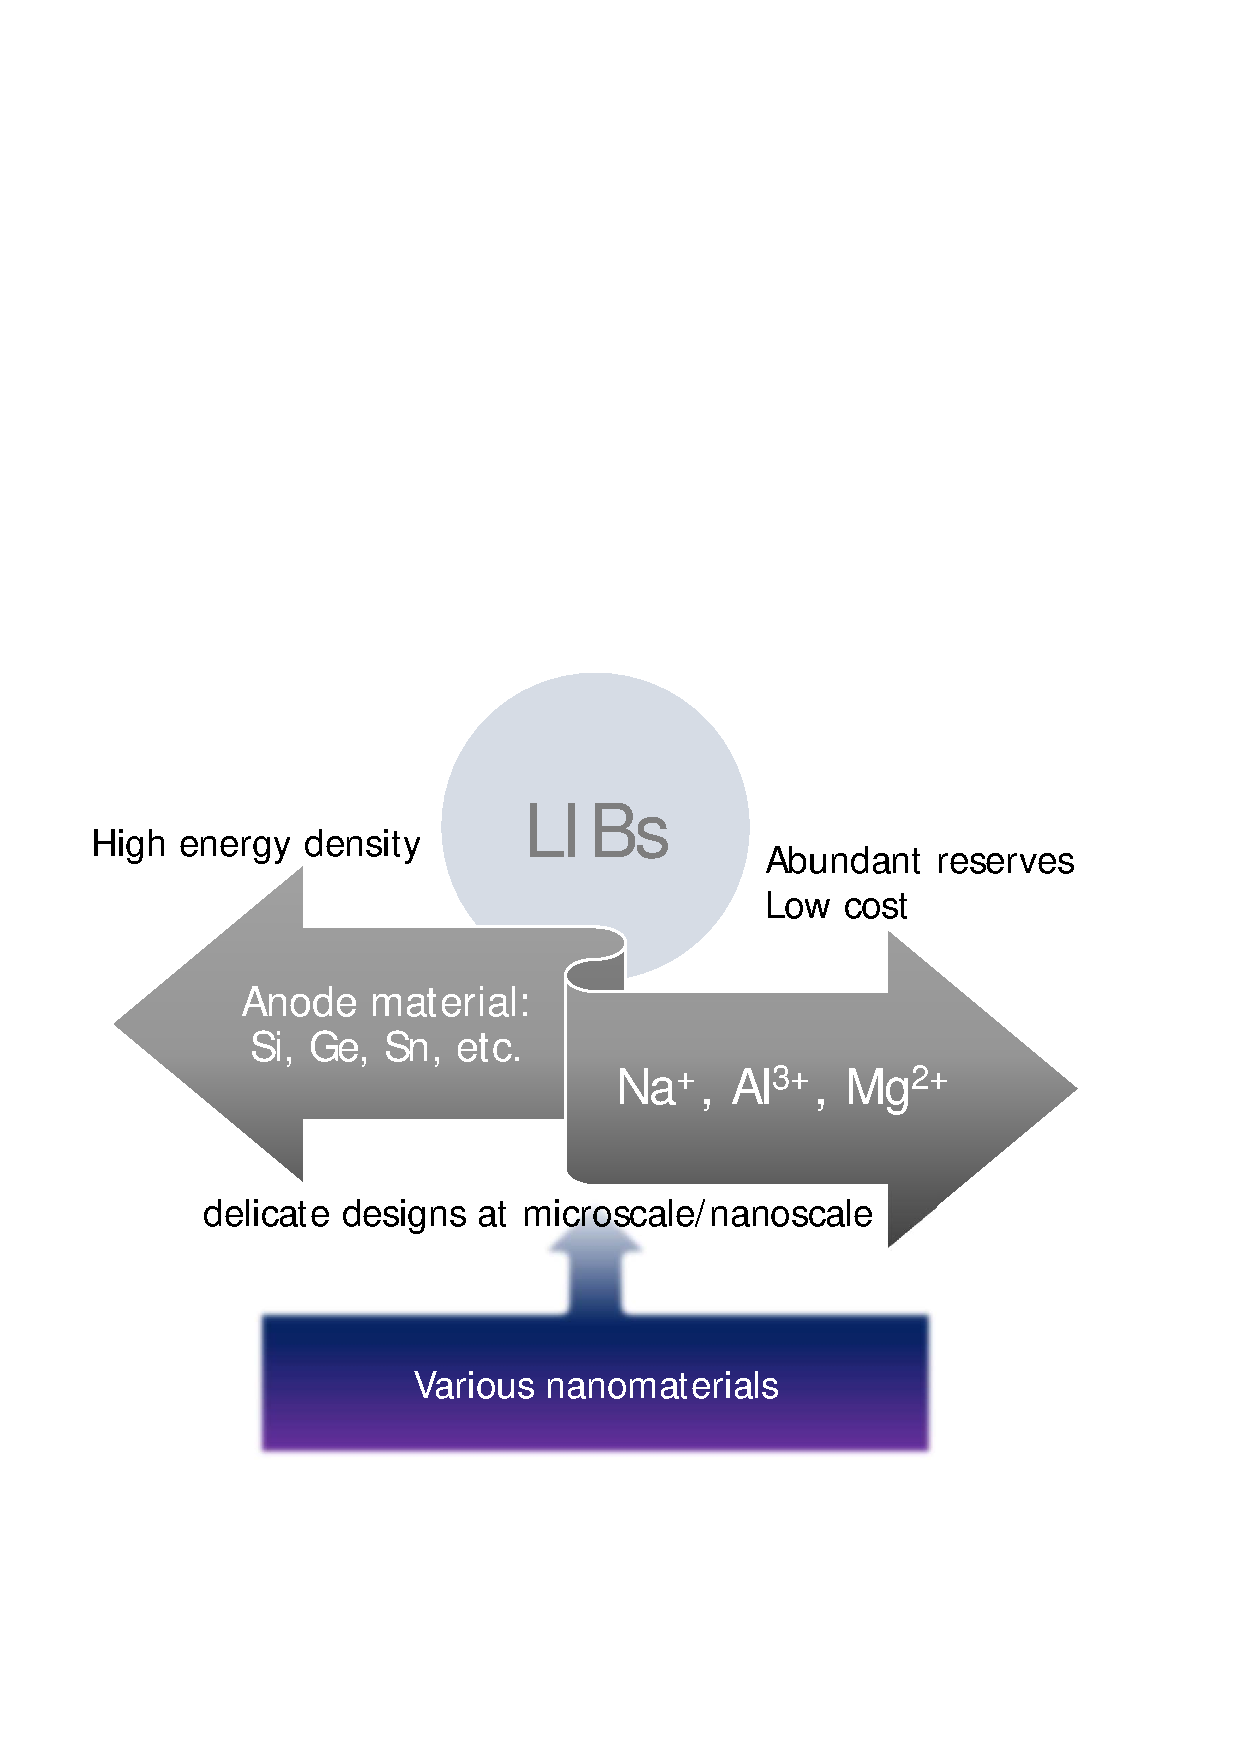
\includegraphics[width=280pt]{figures/figure1_lib.pdf}
\caption[Future of optoelectronics and flexible electroncis]{Silicon's two short-backs for flexible devices and optoelectronics could be backed-up by bottom-up approach using nanomaterials in future integrations.
\label{fig:1lib}}
\end{figure}

%silicon for ion battery anode
 Graphite has widely been the anode of choice for commercial products, since the first generation Li-ion chemistry. Due to strong request of high capacity, recent years, researchers are interested in developing silicon anode material for high capacity lithium-ion batteries. Among all investigated anode materials, silicon has a theoretical capacity of $3590 \mathrm{mAh/g}$ (about 10 times higher than carbon) based on the fully alloyed form of \ce{Li15Si4} at room temperature (at high temperature \ce{Li15Si4} can be reached, giving a capacity of $4200 \mathrm{mAh g−1}$, placing it on top of all other anode materials. In addition, Si anodes show moderate working potential at $0.5$ V, which is higher than graphite anodes at $0.05 $ V. Which means silicon is suitable to solve the safety problem of lithium deposition upon cell overcharge as well as avert the energy penalty of battery cells assembled with the \ce{Li4Ti5O12} anodes.\\
 However, the insertion/extraction of lithium ions result in significant volume change - about 370\% - which leads to structural pulverization and electrical disconnection between anode materials and current collector, and finally the battery lose most functions. Some recent designs of LIBs using silicon materials as anodes allows the battery to maintain anode structure and hence to reach high capacity while at the same time good stablity. 
 
\begin{figure}  
\centering
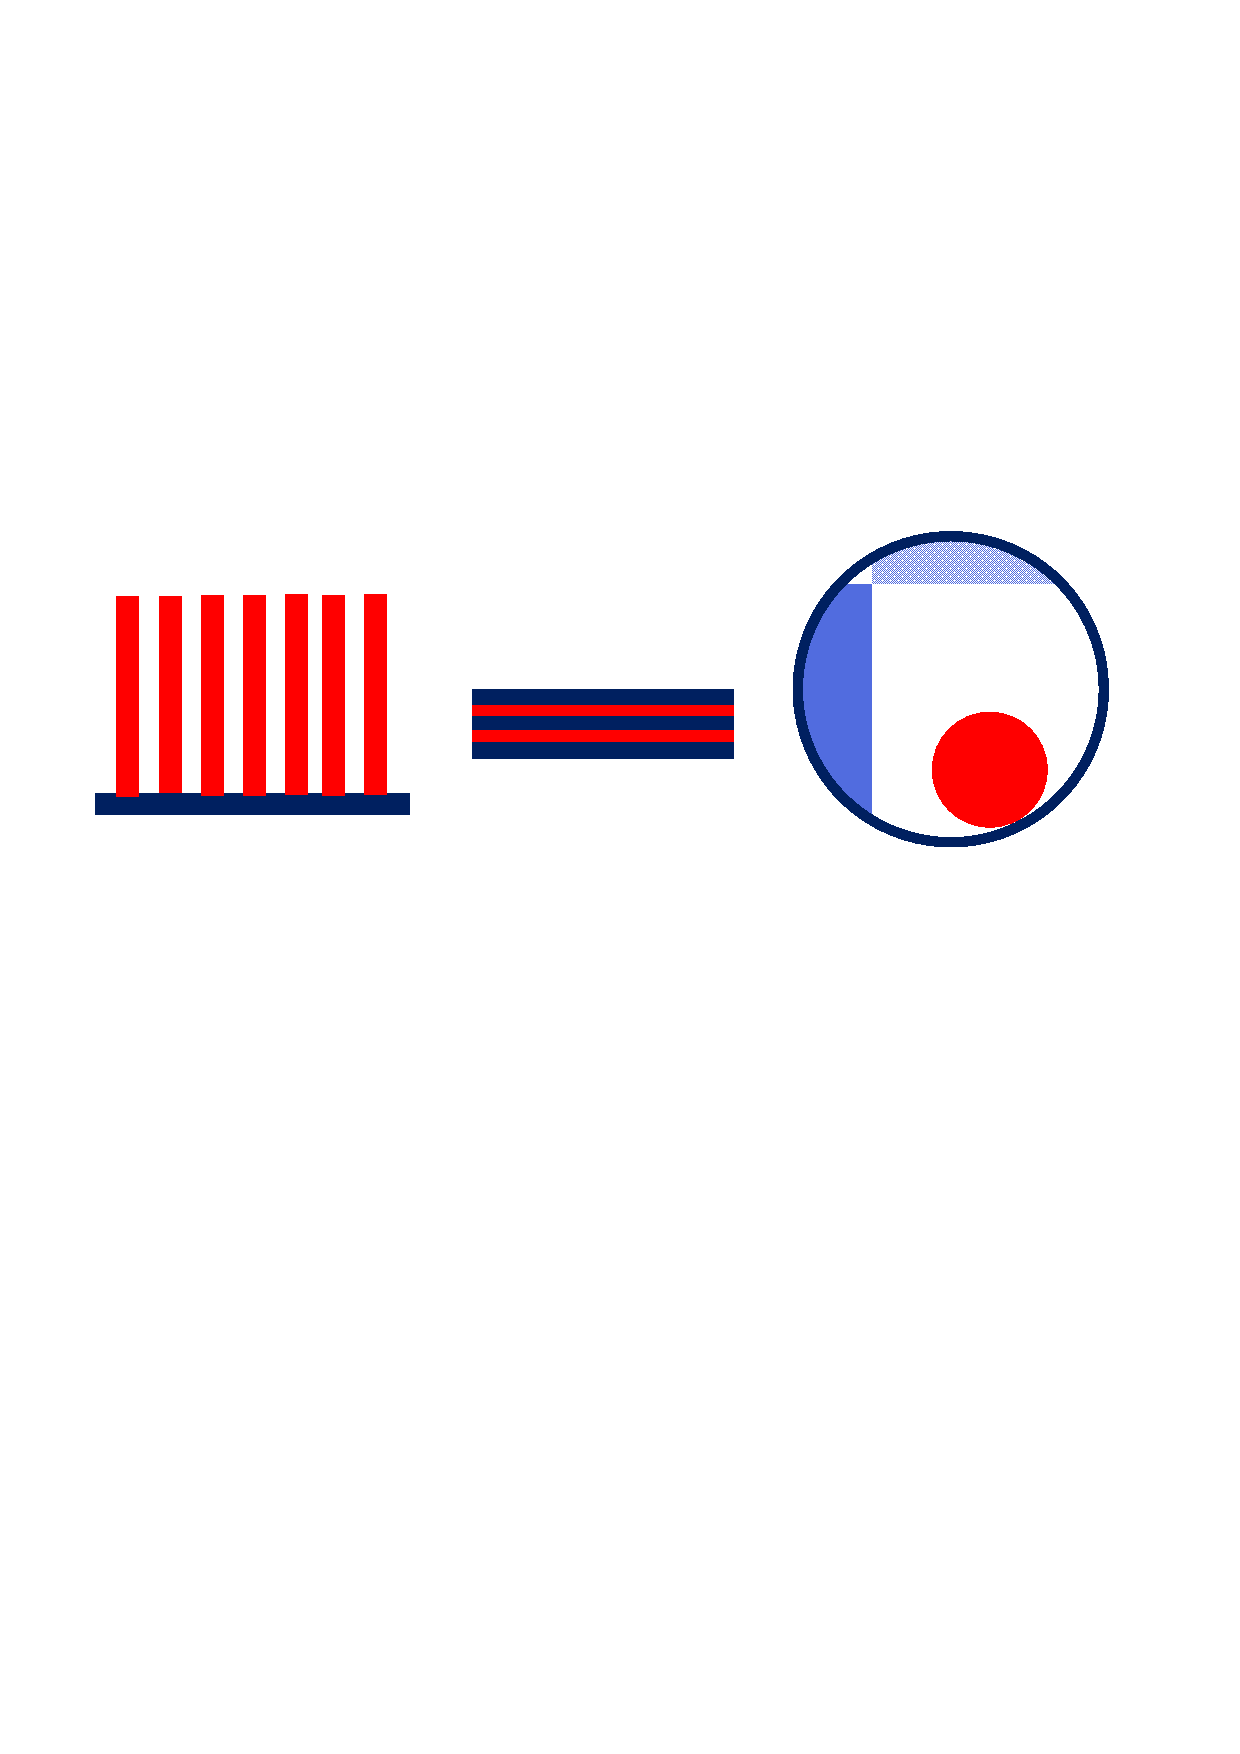
\includegraphics[width=350pt]{figures/figure1_silibdesign}
\caption[Designs for large volume expansion anode materials]{Designs for large volume expansion anode materials in batteries. Red correspond to material with large volume expansion/shrinking during cycling, while material in blue color is the confinement material with low volume expansion rate and good mechanical strength. 
\label{fig:1silibdesign}}
\end{figure}

 Cui et al. designed high performance anode structure by silicon nanowires, which was able to accommodate large strain caused by lithium ion insertion and extraction.\cite{Cui2009} 
 Deng et al. reported a tubular configuration made from rolled-up C/Si/C layered nanomembranes which performs a highly reversible capacity at approximately 2000 mAh /g (50 mA/g), and approximately 100\% capacity retention (500 mA/g) after 300 cycles.\cite{Deng2013}
 Cui et al. also designed core-shell structures for silicon material based LIBs. They proposed a hierarchical structured silicon anode which is inspired by the structure of a pomegranate. The silicon nanoparticles are encapsulated by conductive carbon coatings that leaves just enough space for the expansion and contraction during lithiation and delithiation cycling. \cite{Liu2014d}
 
Therefore, by designing on the microcosmic structures, we are able to utilize the high capacity material with structural and mechanical restrictions, as illustrated in Figure \ref{fig:1silibdesign}. Also, many other attempts of combining silicon with carbon materials, with polimers, with metals, which is summarized by Liang et al.\cite{Liang2014} 
 
%Na-ion batteries
It is predicted that lithium would be the next petroleum resource that will die out.\cite{Jaskula2016} According to the distribution of lithium on earth\cite{Jaskula2011}, Chile could be the next Saudi Arabia. This problem is more essential for many countries with very limited lithium reserves such as Japan.  In order to explore the next generation of secondary batteries, which is called post-lithium ion secondary batteries, many investigations
shows that the most promising candidate is the sodium-ion battery (SIB). SIB uses sodium instead of lithium as the charge carrier, and use iron, manganese and other transition metals to replcae cobalt for redox reactions. If SIBs are expected to be manufactured in mass production due to its
environmental impact and low cost.

\begin{table}[ht]
\centering % used for centering table
\begin{tabular}{|l|c|c|} % left, centered columns (3 columns)
\hline %inserts double horizontal lines
 & LIB & SIB\\ [0.5ex] % inserts table heading
\hline % inserts single horizontal line
Theoretical capacity & 3,829 mAh/g & 1,165 mAh/g \\[1.5ex] % inserting body of the table
Cost (carbonate) & 5,000 USD/t & 150 USD/t \\[1.5ex]% [1.5ex] adds vertical space
Reserves & 23,000 ppm & 20 ppm \\[1.5ex]
Potential & –3.045 V & –2.714 V \\[1.5ex]
Ionic radii & 79.3 pm & 100.9 pm \\[1.5ex]
\hline %inserts single line
\end{tabular}
\caption{Compare LIB and SIB.} % title of Table
\label{table1.1} % is used to refer this table in the text
\end{table}

As shown in Table \ref{table1.1}, even sodium process higher normal electrode potential of ~0.3 V, larger effective radius than lithium (in volume ratio 2.05), smaller theoretical capacity, the cost and environmental benefits are still very attractive for applications does not require very high capacity. Actually, it is hard for graphite, which is commercially used as a anode material for LIBs, to store and release sodium ions both theoretically and in practice because of the size of sodium ion is large. It was discovered in 2000 that hard carbon having disordered structures could electrochemically store and release sodium ions.\cite{Stevens2000} Several
years ago, work was being done on developing and making practical sodium ion batteries, and recently researchers are investigating on many anode active materials for sodium ions. The guidelines and experience from searching electrode active materials for LIBs are not applicable
for SIBs.\cite{Lang2010,Armand2008,KUZE2013}

Consequently, two important research areas of secondary batteries are: better anode active materials with higher capacities, and find other elements for ion batteries, as illustrated in Figure \ref{fig:1lib}. To apply these elements in secondary batteries, nanomaterials, or nanoscaled designs play very important roles - to enable reactions, to overcome huge volumn expansion, to decrease diffusion lengths; while bulk materials are not capable to reach the highest capacity for LIBs nor special ion-batteries at the moment. 

\section{Motivation of my PhD research}
As stated above, {\em in situ} studies for namonaterials toward optoelectronic, electronic and ion batteries are required by the society. My motivation is to take the challenge and analyze the dynamics of the building blocks as well as heterostructures to provide knowledge for advanced applications. 
Therefore, I explored some experimental methods and engineering details in Chapter 2, including {\em in situ} TEM setups and the working mechanisms. Chapter 3 is the first experimental Chapter introducing manipulation possibilities in the frame of the general “nanoarchitectonics” concept and its applications for nanoengineering. The experiments have been performed on the {\em in situ} TEM constructed axial nanowire junctions of CdS and p-Si. Then, detailed electrical probing for energy storage research is discussed in Chapter 4. I fabricated an ultra-stable sodium ion battery and analyzed the mechanism of its cycling performance under {\em in situ} TEM probing. Through coupling with {\em in situ} TEM applied mechanical forces, two examples of force driven optoelectronic phenomena are detailed in Chapter 5 and Chapter 6. 